\chapter{Research question}

The point of this bachelor thesis is to conduct research into chatbots and how they are built. What actually goes into building a chatbot that feels intuitive but is also functional?

\section{Approach}

This thesis will start with some use cases for chatbots. When it would be a good idea to build a chatbot as a solution for a concrete problem.

Already existing chatbots will be presented and compared to paint a picture of what a professional chatbot currently looks like.
Some general research into chatbot best practices and worst practices will also be conducted based on these real life cases and studies.

Finally, different platforms and frameworks to create a fully-fledged chatbot will be compared by building one.

\section{Metrics}

The metrics for the comparison will be based on a couple of different factors. Their general business model will be researched, followed up by their learning curve and quality of documentation. Finally source code readability and scalability will be compared.

\chapter{General chatbot design}

\section{Choosing a chatbot solution}

\subsection{Introduction}

Why choose a chatbot as a solution to a problem? To find the answer to that question there should be a concrete description of the problem and research should be conducted into how that problem is currently handled.

\subsection{Use case 1: Food delivery}

Food delivery chatbots are some of the most common chatbots out there. That's because a basic chatbot for ordering food is easy to make and maintain. Most of the time they don't require complex language recognition and they will go through the same steps every time someone wants to order something.

A great example of this is Domino's. They own one of the most popular facebook messenger chatbots even though the bot itself is really simple.

Taking a look at the perspective of a new imaginary pizza place in town. This pizza place has a set menu with set formulas. They want to innovate and make it possible to receive and process online orders but don't want to lose the familiarity of their brand.

This is a perfect case for a chatbot. If they already have a facebook page, they can easily integrate a chatbot into it and promote it to their current customers. All they need on top of that is an admin panel for the company to maintain their menu and process orders.

Building a chatbot this way also opens up several possibilities for expansion in the future. They can easily start tracking customer's habits and improve their suggestions for specific customers.

There are some downsides to this solution as well however. Creating a chatbot from scratch for this purpose would cost a lot of money. That's why there are already solutions like Chatobook~\cite{chatobook} popping up. This is an all-in-one solution that provides a restaurant with a messenger bot and an admin panel to manage promotion, reservations and the menu. You can also find templates for these kinds of bots that integrate with Google Sheets/Excel.~\cite{chatbot-templates-pizza}

The rise of general delivery services like Ubereats~\cite{ubereats} and Deliveroo~\cite{deliveroo} also complicates this matter. If those companies manage to integrate full ordering services into their platforms using chatbots -which they will most likely succeed in at one point- that would simplify everything. But that also comes with a cost. The imaginary pizza restaurant would lose their unique identity as the chatbot's identity would be replaced with Uber's or Deliveroo's identity.

\subsection{Use case 2: Banking industry}

Next up is the banking industry. Lately there has been an influx of integrating AI-powered chatbots into this sector. This is because people like to engage with their bank and get answers that feel human, instantly. It establishes a form of trust. This form of communication is also very attractive to the banks themselves, because it allows them to quickly provide answers to repetitive questions.

There's lots of specific chatbot banking use cases out there. One of them is simply basic banking services. Checking account balance, transferring funds, analyzing expenditures. Chatbots can also hugely improve a bank's customer support, which should be available 24/7. They can help out people instantly, without long wait times which a lot of customer support services are currently struggling with. Further more, there's also the opportunity for intranet-based chatbots~\cite{intranet-chabot}. These chatbots communicate with the employees to improve their productivity and give them access to the right information in mere seconds. Another use case is the delivery of customer-focused marketing. Using a chatbot, it's easier to promote personalized banking services as if the customer is talking to a real life employee.

Overall, integrating a chatbot into a banking environment has lots of benefits. That's why more and more banks are starting to invest in them.

\subsection{Use case 3: E-commerce}

Lastly there's the quickly growing industry of E-commerce. This ties into both of the use cases above as the main focus is customer interaction and engagement, support and personalized marketing.

Online web-stores are one of the fastest growing industries out there, they are popping up everywhere. This is because more and more people are starting to buy online. It's convenient, fast and reliable (in most cases). However there is one key benefit missing compared to in-store shopping; interaction.

In comes the shopping assistant chatbot. It can do everything a normal store employee can and more. Like instantly retrieving your past orders to help you out quicker and more efficiently. It can have access to every single product the web-shop offers and instantly recommend one that fits your needs. It can seamlessly provide post-purchase customer support. All of this whilst not losing the brand identity of the web-store in question.

\subsection{Conclusion}

Chatbots are an obvious answer to lots of companies that are starting to innovate and are ready to experiment. It allows for them to establish their brand in a familiar and human way, whilst also increasing their in-company productivity and overall efficiency.

\begin{figure}[p]
  \centering
  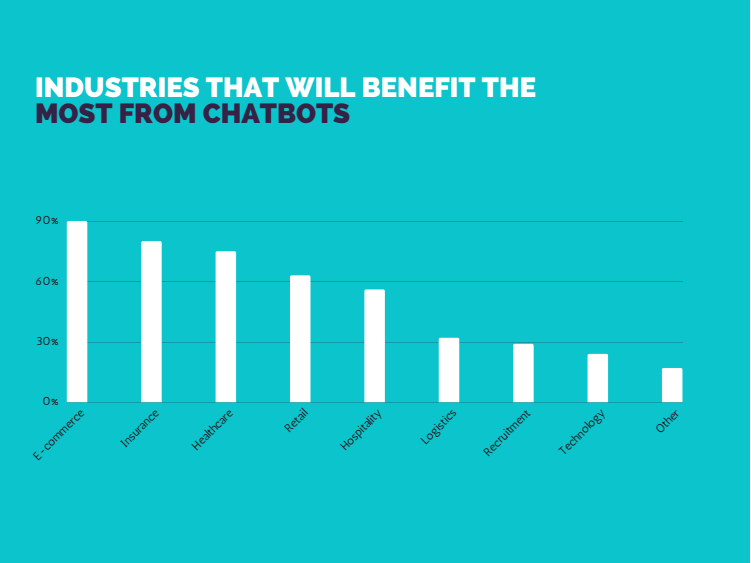
\includegraphics[width=\textwidth]{chatbot-benefit-graph2}\label{fig:chatbot-benefit-graph2}
  \caption{Industries projected to benefit from chatbots~\cite{chatbot-industry-benefits}}
\end{figure}

\begin{figure}[p]
  \centering
  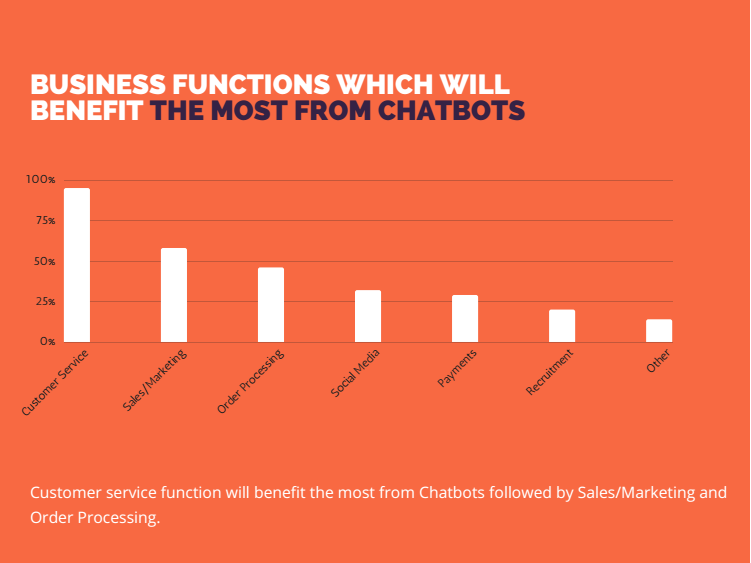
\includegraphics[width=\textwidth]{chatbot-benefit-graph}\label{fig:chatbot-benefit-graph}
  \caption{Business functions inside a company projected to benefit from chatbots~\cite{chatbot-industry-benefits}}
\end{figure}

\newpage

\section{Comparison of existing chatbots}

Today there are plenty of well-implemented solutions already. There's food-ordering services like Domino's that have their very popular messenger chatbot. But also stores ranging from specific ones (H\&M) to big fully fledged web-stores like Bol.com, a Dutch-Belgian web-store.

\subsection{Dom, Domino's ordering assistant bot}

This is a facebook messenger bot for ordering food from Domino's, a fast food chain. Something you immediately notice is the use of tappable quick reply answers. The bot starts of with some simple questions to establish the user's intent and some information about the user like the address and what store he or she wants to order from.

Once this has been established, the user can choose what he wants to order and checkout.

All in all, the bot is pretty simplistic. It takes orders and passes them through to the store. There's a lot of room for improvement here. The bot could in theory build a profile of you using your past orders and recommend you an order off the bat. It could also keep you updated on new items being released. On top of that it seems the bot isn't very smart yet. The user needs to follow the steps clearly and in the right order. In general, it doesn't mimic a real life conversation.

In conclusion Dom is a very utility-focused bot. It doesn't aim to connect with the user and spread Domino's brand identity, it's solely focused on the ordering aspect.